\documentclass{beamer}
\usetheme{CambridgeUS}
%%%%%%%%%%%%%%%%%%%%%%%%%%%%%%%%%%%%%%%%%%%%%%%%%%%%%%%
\setbeamercolor{block title}{bg=red!80!black, fg=white}
\setbeamercolor{block body}{bg=red!10, fg=black}
%%%%%%%%%%%%%%%%%%%%%%%%%%%%%%%%%%%%%%%%%%%%%%%%%%%%%%%
\usepackage[utf8]{vietnam}
\usepackage{tikz}
\usepackage{calc}
\usepackage{hyperref}
\usepackage{graphicx}
\usepackage{lipsum}
\usepackage{bookmark}
\usepackage{amsmath}
\usepackage{amssymb}

%%%%%%%%%%%%%%%%%%%%%%%%%%%%%%%%%%%%%%%%%%%%%%%%%%%%%%%
% Định nghĩa đánh công thức có số chương
\numberwithin{equation}{section}
\AtBeginSection[]{
\setcounter{section}{\thesection}
\refstepcounter{section}
}
%%%%%%%%%%%%%%%%%%%%%%%%%%%%%%%%%%%%%%%%%%%%%%%%%%%%%%%
\AtBeginSection[]
{
\begin{frame}<beamer>
\frametitle{Nội dung}

\tableofcontents[
currentsection,
subsectionstyle=hide/hide,
subsubsectionstyle=hide/hide
]
\end{frame}
}
%%%%%%%%%%%%%%%%%%%%%%%%%%%%%%%%%%%%%%%%%%%%%%%%%%%%%%%
\title[{\makebox[.15\paperwidth]{MI4100 - Mật mã và độ phức tạp thuật toán}}]{Chủ đề: Mô phỏng tấn công hệ mật mã khóa công khai RSA bằng thuật toán LLL giảm lưới}
\author[Nhóm 8]{Nhóm 8}
\date[\today]{\today}
%%%%%%%%%%%%%%%%%%%%%%%%%%%%%%%%%%%%%%%%%%%%%%%%%%%%%%%
\begin{document}
%%%%%%%%%%%%%%%%%%%%%%%%%%%%%%%%%%%%%%%%%%%%%%%%%%%%%%%
% Trang tiêu đề cần có hình ảnh pictures/HUST2.jpeg
% Không chỉnh sửa gì
\begin{frame}
\begin{tikzpicture}[remember picture, overlay]
\node[anchor=center, inner sep=0pt] at (current page.center) {
\includegraphics[width=\paperwidth, height=\paperheight]{pictures/HUST2.jpeg}};
\fill[white, opacity=0.8] (current page.south west) rectangle (current page.north east);
\end{tikzpicture}
\titlepage
\end{frame}
%%%%%%%%%%%%%%%%%%%%%%%%%%%%%%%%%%%%%%%%%%%%%%%%%%%%%%%
%! %%%%%%%%%%%%%%%%%%%%%%%%%%%%%%%%%%%%%%%%%%%%%%%%%%%%%%
%! %%%%%%%%%%%%%%%%%%%%%%%%%%%%%%%%%%%%%%%%%%%%%%%%%%%%%%
%! %%%%%%%%%%%%%%%%%%%%%%%%%%%%%%%%%%%%%%%%%%%%%%%%%%%%%%
%! %%%%%%%%%%%%%%%%%%%%%%%%%%%%%%%%%%%%%%%%%%%%%%%%%%%%%%
%! %%%%%%%%%%%%%%%%%%%%%%%%%%%%%%%%%%%%%%%%%%%%%%%%%%%%%%
\section{Phương pháp lưới và thuật toán LLL}
\subsection{Phương pháp lưới}
%%%%%%%%%%%%%%%%%%%%%%%%%%%%%%%%%%%%%%%%%%%%%%%%%%%%%%%
% Survey: Lattice Reduction Attacks on RSA; David Wong; supervised by Guilhem Castagnos; University of Bordeaux, March 2015
\begin{frame}{Giới thiệu về lưới}

\begin{itemize}
\item Lưới tương tự như không gian vector.
\item Ví dụ không gian vector đơn giản gồm 2 vector. Bạn có thể cộng, nhân với số vô hướng và nó trải rộng trong một không gian vector.
\end{itemize}

\resizebox{0.9\textwidth}{!}{%

\begin{tikzpicture}[scale=.55]
\draw [lightgray] [<->] (0, 5) -- (10, 5);
\draw [lightgray] [<->] (5, 10) -- (5, 0);
\draw [thick, purple] [->] (5, 5) -- (6, 8);
\draw [thick, purple] [->] (5, 5) -- (6, 6);

\draw [thick, black] [->] (11, 5) -- (12, 5);

\draw [lightgray] [<->] (13, 5) -- (23, 5);
\draw [lightgray] [<->] (18, 10) -- (18, 0);
\path [fill=purple] (15.5, 0) to (20.5, 10) to (23, 10) to (13, 0);
\end{tikzpicture}
}

\end{frame}
%%%%%%%%%%%%%%%%%%%%%%%%%%%%%%%%%%%%%%%%%%%%%%%%%%%%%%%
% Survey: Lattice Reduction Attacks on RSA; David Wong; supervised by Guilhem Castagnos; University of Bordeaux, March 2015
\begin{frame}{Giới thiệu về lưới}

\begin{itemize}
\item Tuy nhiên các số vô hướng của lưới là các số nguyên.
\item Bây giờ ta có không gian được tạo thành từ các điểm.
\end{itemize}

\begin{figure}[!h]
\centering
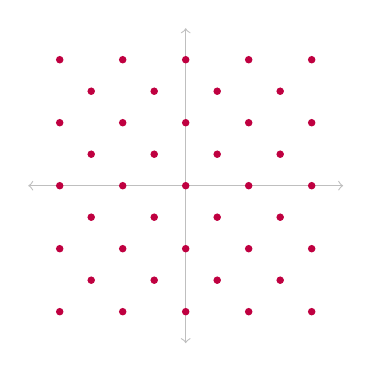
\begin{tikzpicture}[scale=.4]
\draw [lightgray] [<->] (0, 5) -- (10, 5);
\draw [lightgray] [<->] (5, 10) -- (5, 0);

\draw [fill, purple] (9, 1) circle [radius=0.1];

\draw [fill, purple] (7, 1) circle [radius=0.1];
\draw [fill, purple] (8, 2) circle [radius=0.1];
\draw [fill, purple] (9, 3) circle [radius=0.1];

\draw [fill, purple] (5, 1) circle [radius=0.1];
\draw [fill, purple] (6, 2) circle [radius=0.1];
\draw [fill, purple] (7, 3) circle [radius=0.1];
\draw [fill, purple] (8, 4) circle [radius=0.1];
\draw [fill, purple] (9, 5) circle [radius=0.1];

\draw [fill, purple] (3, 1) circle [radius=0.1];
\draw [fill, purple] (4, 2) circle [radius=0.1];
\draw [fill, purple] (5, 3) circle [radius=0.1];
\draw [fill, purple] (6, 4) circle [radius=0.1];
\draw [fill, purple] (7, 5) circle [radius=0.1];
\draw [fill, purple] (8, 6) circle [radius=0.1];
\draw [fill, purple] (9, 7) circle [radius=0.1];

\draw [fill, purple] (1, 1) circle [radius=0.1];
\draw [fill, purple] (2, 2) circle [radius=0.1];
\draw [fill, purple] (3, 3) circle [radius=0.1];
\draw [fill, purple] (4, 4) circle [radius=0.1];
\draw [fill, purple] (5, 5) circle [radius=0.1];
\draw [fill, purple] (6, 6) circle [radius=0.1];
\draw [fill, purple] (7, 7) circle [radius=0.1];
\draw [fill, purple] (8, 8) circle [radius=0.1];
\draw [fill, purple] (9, 9) circle [radius=0.1];

\draw [fill, purple] (1, 3) circle [radius=0.1];
\draw [fill, purple] (2, 4) circle [radius=0.1];
\draw [fill, purple] (3, 5) circle [radius=0.1];
\draw [fill, purple] (4, 6) circle [radius=0.1];
\draw [fill, purple] (5, 7) circle [radius=0.1];
\draw [fill, purple] (6, 8) circle [radius=0.1];
\draw [fill, purple] (7, 9) circle [radius=0.1];

\draw [fill, purple] (1, 5) circle [radius=0.1];
\draw [fill, purple] (2, 6) circle [radius=0.1];
\draw [fill, purple] (3, 7) circle [radius=0.1];
\draw [fill, purple] (4, 8) circle [radius=0.1];
\draw [fill, purple] (5, 9) circle [radius=0.1];

\draw [fill, purple] (1, 7) circle [radius=0.1];
\draw [fill, purple] (2, 8) circle [radius=0.1];
\draw [fill, purple] (3, 9) circle [radius=0.1];

\draw [fill, purple] (1, 9) circle [radius=0.1];
\end{tikzpicture}
\end{figure}

\begin{block}{Nhận xét}
Lưới rất hữu ích trong mật mã vì chúng mang lại cho chúng ta rất nhiều công cụ để xử lý các số nguyên.
\end{block}

\end{frame}
%%%%%%%%%%%%%%%%%%%%%%%%%%%%%%%%%%%%%%%%%%%%%%%%%%%%%%%
\begin{frame}{Định nghĩa lưới}

\begin{block}{Định nghĩa lưới}

Cho \(n \geq 1 \), \(\{x_1, x_2, \ldots, x_n\}\) là một cơ sở của \(\mathbb{R}^n\).
Lưới \(n \) chiều với cơ sở \(\{x_1, x_2, \ldots, x_n\}\)
là tập hợp \(L \) tất cả các tổ hợp tuyến tính của các vector cơ sở đó với hệ số nguyên:

$$
L = \{a_1 x_1 + a_2 x_2 + \ldots + a_n x_n \mid a_i \in \mathbb{Z} \}
$$

Các vector \(\{x_1, x_2, \ldots, x_n\}\) được gọi là cơ sở của lưới.

\end{block}

\end{frame}
%%%%%%%%%%%%%%%%%%%%%%%%%%%%%%%%%%%%%%%%%%%%%%%%%%%%%%%
\begin{frame}{Ví dụ về lưới 2 chiều}

% # Ví dụ về lưới 2 chiều
% # ta có 2 vector cở sở là b1 b2
% # và tập các điểm rời rạc của lưới được tạo từ vector cơ sở
% # Ví dụ như b3 = -b1; b4=b1+b2

\begin{figure}[!h]
\centering
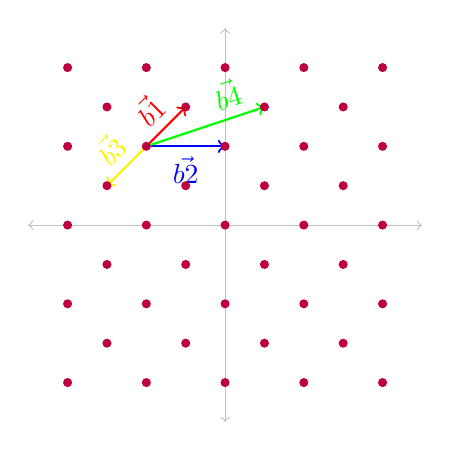
\begin{tikzpicture}[scale=.5]
\draw [lightgray] [<->] (0, 5) -- (10, 5);
\draw [lightgray] [<->] (5, 10) -- (5, 0);

\draw[->, thick, red] (3, 7) -- (4, 8) node[midway, above, sloped] {$\vec{b1}$};
\draw[->, thick, blue] (3, 7) -- (5, 7) node[midway, below, sloped] {$\vec{b2}$};
\draw[->, thick, yellow] (3, 7) -- (2, 6) node[midway, above, sloped] {$\vec{b3}$};
\draw[->, thick, green] (3, 7) -- (6, 8) node[pos=0.75, above, sloped] {$\vec{b4}$};

\draw [fill, purple] (9, 1) circle [radius=0.1];

\draw [fill, purple] (7, 1) circle [radius=0.1];
\draw [fill, purple] (8, 2) circle [radius=0.1];
\draw [fill, purple] (9, 3) circle [radius=0.1];

\draw [fill, purple] (5, 1) circle [radius=0.1];
\draw [fill, purple] (6, 2) circle [radius=0.1];
\draw [fill, purple] (7, 3) circle [radius=0.1];
\draw [fill, purple] (8, 4) circle [radius=0.1];
\draw [fill, purple] (9, 5) circle [radius=0.1];

\draw [fill, purple] (3, 1) circle [radius=0.1];
\draw [fill, purple] (4, 2) circle [radius=0.1];
\draw [fill, purple] (5, 3) circle [radius=0.1];
\draw [fill, purple] (6, 4) circle [radius=0.1];
\draw [fill, purple] (7, 5) circle [radius=0.1];
\draw [fill, purple] (8, 6) circle [radius=0.1];
\draw [fill, purple] (9, 7) circle [radius=0.1];

\draw [fill, purple] (1, 1) circle [radius=0.1];
\draw [fill, purple] (2, 2) circle [radius=0.1];
\draw [fill, purple] (3, 3) circle [radius=0.1];
\draw [fill, purple] (4, 4) circle [radius=0.1];
\draw [fill, purple] (5, 5) circle [radius=0.1];
\draw [fill, purple] (6, 6) circle [radius=0.1];
\draw [fill, purple] (7, 7) circle [radius=0.1];
\draw [fill, purple] (8, 8) circle [radius=0.1];
\draw [fill, purple] (9, 9) circle [radius=0.1];

\draw [fill, purple] (1, 3) circle [radius=0.1];
\draw [fill, purple] (2, 4) circle [radius=0.1];
\draw [fill, purple] (3, 5) circle [radius=0.1];
\draw [fill, purple] (4, 6) circle [radius=0.1];
\draw [fill, purple] (5, 7) circle [radius=0.1];
\draw [fill, purple] (6, 8) circle [radius=0.1];
\draw [fill, purple] (7, 9) circle [radius=0.1];

\draw [fill, purple] (1, 5) circle [radius=0.1];
\draw [fill, purple] (2, 6) circle [radius=0.1];
\draw [fill, purple] (3, 7) circle [radius=0.1];
\draw [fill, purple] (4, 8) circle [radius=0.1];
\draw [fill, purple] (5, 9) circle [radius=0.1];

\draw [fill, purple] (1, 7) circle [radius=0.1];
\draw [fill, purple] (2, 8) circle [radius=0.1];
\draw [fill, purple] (3, 9) circle [radius=0.1];

\draw [fill, purple] (1, 9) circle [radius=0.1];
\end{tikzpicture}
\end{figure}
\end{frame}
%%%%%%%%%%%%%%%%%%%%%%%%%%%%%%%%%%%%%%%%%%%%%%%%%%%%%%%
% # ??????????????? Nguyên, +-1, det,
%%%%%%%%%%%%%%%%%%%%%%%%%%%%%%%%%%%%%%%%%%%%%%%%%%%%%%%
\subsection{Quy trình Gram-Schmidt}
\begin{frame}{Quy trình Gram-Schmidt}

\begin{itemize}
\item Quy trình Gram-Schmidt chuyển một cơ sở bất kỳ thành một cơ sở trực giao.
\item Đây là kỹ thuật quan trọng trong thuật toán LLL.
\end{itemize}

\begin{columns}

\begin{column}{0.5\textwidth}
\begin{figure}[h]

\resizebox{0.9\textwidth}{!}{%

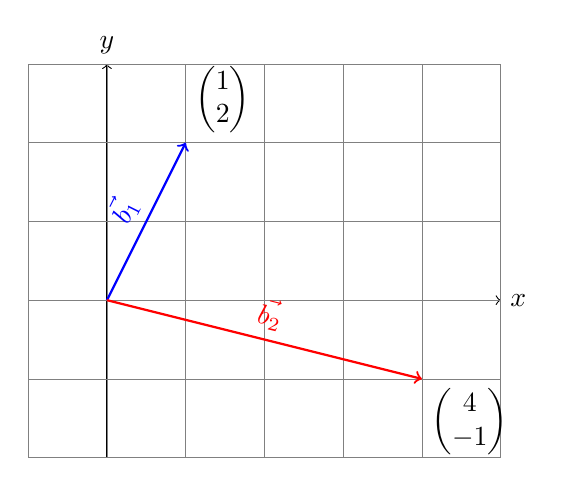
\begin{tikzpicture}
% Vẽ trục tọa độ
\draw[->] (-1, 0) -- (5, 0) node[right] {$x$};
\draw[->] (0, -2) -- (0, 3) node[above] {$y$};

% Vẽ lưới
\draw[very thin, gray] (-1, -2) grid (5, 3);

% Vẽ vector (1, 2)
\draw[->, thick, blue] (0, 0) -- (1, 2) node[midway, above, sloped] {$\vec{b_1}$};

% Vẽ vector (4, -1)
\draw[->, thick, red] (0, 0) -- (4, -1) node[midway, above, sloped] {$\vec{b_2}$};

% Gắn nhãn điểm cuối vector
\node at (1, 2) [above right] {$\begin{pmatrix} 1 \\ 2 \end{pmatrix}$};
\node at (4, -1) [below right] {$\begin{pmatrix} 4 \\ -1 \end{pmatrix}$};
\end{tikzpicture}

}

\end{figure}
\end{column}

\begin{column}{0.5\textwidth}
\begin{figure}[h]

\resizebox{0.9\textwidth}{!}{%

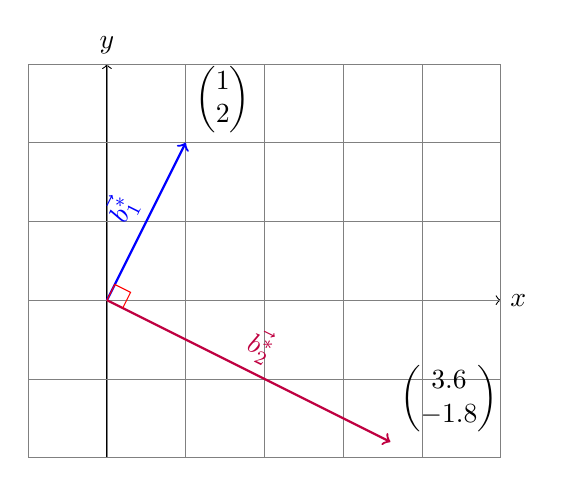
\begin{tikzpicture}
% Vẽ trục tọa độ
\draw[->] (-1, 0) -- (5, 0) node[right] {$x$};
\draw[->] (0, -2) -- (0, 3) node[above] {$y$};

% Vẽ lưới
\draw[very thin, gray] (-1, -2) grid (5, 3);

% Vẽ vector (1, 2)
\draw[->, thick, blue] (0, 0) -- (1, 2) node[midway, above, sloped] {$\vec{b_1^*}$};

% Vẽ vector (3.6, -1.8)
\draw[->, thick, purple] (0, 0) -- (3.6, -1.8) node[midway, above, sloped] {$\vec{b_2^*}$};

% Gắn nhãn điểm cuối vector
\node at (1, 2) [above right] {$\begin{pmatrix} 1 \\ 2 \end{pmatrix}$};
\node at (3.6, -1.8) [above right] {$\begin{pmatrix} 3.6 \\ -1.8 \end{pmatrix}$};

% Vẽ ký hiệu vuông góc màu đỏ tại gốc tọa độ
\draw[red] (0, 0) -- (0.1, 0.2) -- (0.3, 0.1) -- (0.2, -0.1);
\end{tikzpicture}

}

\end{figure}
\end{column}

\end{columns}

\end{frame}
%%%%%%%%%%%%%%%%%%%%%%%%%%%%%%%%%%%%%%%%%%%%%%%%%%%%%%%
\begin{frame}{Quy trình Gram-Schmidt}

\begin{block}{Định nghĩa}

Cho $x_1, x_2, \ldots, x_n$ là một cơ sở trong $\mathbb{R}^n$.
Trực giao hóa Gram-Schmidt của $x_1, x_2, \ldots, x_n$
là một cơ sở $x_1^*, x_2^*, \ldots, x_n^*$ được định nghĩa như sau:

\begin{itemize}
\item $x_1 = x_1^*$,
\item $x_i^* = x_i - \sum_{j=1}^{i-1} \mu_{ij} x_j^*$, \quad $2 \leq i \leq n$, \quad $\mu_{ij} = \frac{\langle x_i, x_j^* \rangle}{\langle x_j^*, x_j^* \rangle}$.
\end{itemize}

\end{block}

\end{frame}
%%%%%%%%%%%%%%%%%%%%%%%%%%%%%%%%%%%%%%%%%%%%%%%%%%%%%%%
\subsection{Thuật toán LLL}
\begin{frame}{Thuật toán LLL}
\begin{itemize}
\item Thuật toán LLL rút gọn cơ sở $B$ của lưới $L$ thành một cơ sở mới $B'$ ngắn hơn sao cho $|\det(L)|$ không đổi.
\item Thuật toán LLL cho kết quả là cơ sở mới ngắn hơn và trực giao hơn

\begin{figure}[H]
\centering
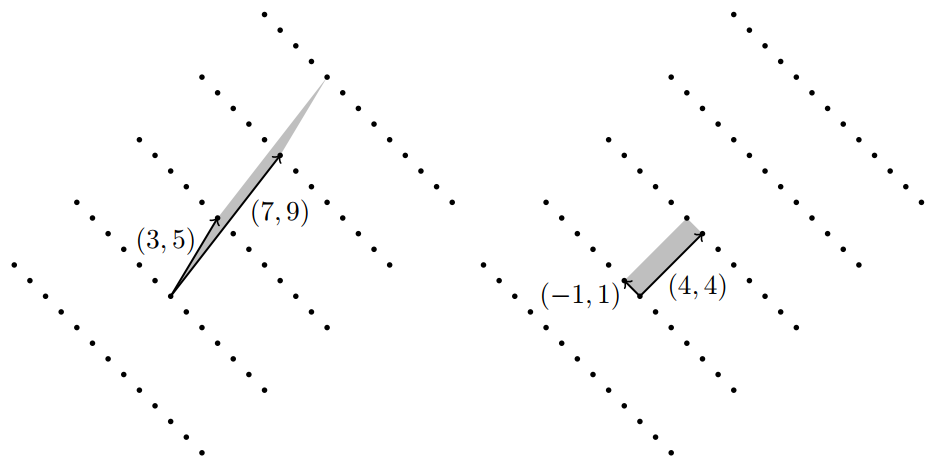
\includegraphics[scale = 0.5]{pictures/mo_ta_ket_qua_giam_luoi_LLL.png}
\caption{Lưới $L \subset R^2$. Mô tả kết quả giảm lưới trong $R^2$.}
\end{figure}

\end{itemize}
\end{frame}
%%%%%%%%%%%%%%%%%%%%%%%%%%%%%%%%%%%%%%%%%%%%%%%%%%%%%%%

% <!-- Điều kiện 1 -->

% <!-- Điều kiện 2 -->

% <!-- Mã giả -->

% <!-- Ví dụ -->

% <!--! Thuật toán LLL -->

% <!-- quy trình Gram-Schmidt: -->
% <!--Nếu $x_1, x_2, \dots, x_n$ là một cơ sở của lưới $L$ thì sau khi trực giao hóa ta thu được các vector $x_1^*, x_2^*, \dots, x_n^*$ có thể không nằm trong lưới $L$. -->
% <!-- Vì num là phân số.... -->
% <!-- Xin chào! Bạn có thể vui lòng giải thích mục đích của dòng: bk = bk - [uk, j]bj là gì không? -->
% <!-- quy trình Gram Schmidt làm cho cơ sở trực giao -->
% <!-- Tuy nhiên, trong LLL chúng ta đang làm việc trong một mạng nên không thể đảm bảo tính trực giao. -->
% <!-- Để làm được điều đó, chúng ta cần u_{k, j} là một số nguyên. -->
% <!-- Điều này tạo ra một cơ sở "đủ trực giao" trong khi vẫn còn trong mạng -->

% <!-- 2 chiều -->
% <!-- n chiều -->
% <!-- Thuật toán LLL giảm lưới -->

%! %%%%%%%%%%%%%%%%%%%%%%%%%%%%%%%%%%%%%%%%%%%%%%%%%%%%%%
%! %%%%%%%%%%%%%%%%%%%%%%%%%%%%%%%%%%%%%%%%%%%%%%%%%%%%%%
%! %%%%%%%%%%%%%%%%%%%%%%%%%%%%%%%%%%%%%%%%%%%%%%%%%%%%%%
%! %%%%%%%%%%%%%%%%%%%%%%%%%%%%%%%%%%%%%%%%%%%%%%%%%%%%%%
%! %%%%%%%%%%%%%%%%%%%%%%%%%%%%%%%%%%%%%%%%%%%%%%%%%%%%%%
\section*{}
\begin{frame}{}
\centering
\Huge{Thanks for listening!}
\end{frame}
%%%%%%%%%%%%%%%%%%%%%%%%%%%%%%%%%%%%%%%%%%%%%%%%%%%%%%%
\end{document}
%%%%%%%%%%%%%%%%%%%%%%%%%%%%%%%%%%%%%%%%%%%%%%%%%%%%%%%

% Lý thuyết
% Lịch sử
% Giới thiệu
% Mục đích công dụng

% Hình ảnh liên quan

% Thuật toán
% Các bước
% Sơ đồ thuật toán

% Code mã nguồn mã giả....

% Ví dụ minh họa
% Chạy tay
% Chương trình lập trình